% arara: pdflatex: { synctex: yes }
% arara: makeindex: { style: ctuthesis }
%% arara: bibtex


%\listfiles


%\PassOptionsToPackage{cp1250}{inputenc}

% The class takes all the key=value arguments that \ctusetup does,
% and couple more: draft and oneside
\documentclass[twoside]{ctuthesis}

\usepackage{graphicx}
\usepackage{svg}
\usepackage{amsmath}
\usepackage{siunitx}
\usepackage{caption}
\usepackage{subcaption}
\usepackage{placeins}
\usepackage{textgreek}
\usepackage{pdfpages}
\usepackage{bytefield}
\usepackage{tikz-timing}
\usepackage{soul}

\usepackage{float}
\usepackage[defernumbers=true, sorting=none]{biblatex}
\addbibresource{bibliography.bib}


\newcolumntype{?}{!{\vrule width 2pt}}

\usepackage{svg}
\svgsetup{
    inkscape=pdf,
    inkscapeexe={C:/inkscape.exe.lnk -z -C"}
}
\graphicspath{{images/}}

\usepackage[per-mode=symbol,separate-uncertainty=true]{siunitx}


\DeclareSIUnit\bit{b}


\makeatletter
\edef\mytoday{\expandafter\@gobbletwo\the\year\ifnum\month<10 0\fi\the\month\ifnum\day<10 0\fi\the\day}
\makeatother

% LaTeX logo with better kerning in sf bf font
\makeatletter
\newcommand\LaTeX@lmss@bx{L\kern -.33em{\sbox \z@ T\vbox to\ht \z@ {\hbox {\check@mathfonts \fontsize \sf@size \z@ \math@fontsfalse \selectfont A}\vss }}\kern -.15em\TeX}
\DeclareRobustCommand\myLaTeX{%
	\ifcsname LaTeX@\f@family @\f@series\endcsname
		\csname LaTeX@\f@family @\f@series\endcsname
	\else
		\LaTeX
	\fi
}

\ctusetup{
%	preprint = {\ctuverlog \\ ctuman \mytoday},
	mainlanguage = english,
	titlelanguage = english,
	otherlanguages = {english},
	title-czech = {Vyčítací systém pro FastIC+},
	title-english = {FastIC+ readout system},
	doctype-english = {Diploma Thesis},
	xfaculty = F3,
        xdoctype = M,
	department-english = {Department of Microelectronics},
%	department-english = {Department of Mathematics},
	author = {Bc. Vojtěch Vosáhlo},
	supervisor = {Ing. Vít Záhlava, CSc.},
        fieldofstudy-english = {Electronics},
%	supervisor-address = {Ústav X, \\ Uliční 5, \\ Praha 99},
	keywords-czech = {FastIC+, Vyčítací systém, Rychlé časování, CERN, DPS},
	keywords-english = {FastIC+, Readout system, Fast Timing, CERN, PCB},
	day = 25,
	month = 5,
	year = 2025,
%	list-of-figures = false,
%	list-of-tables = false,
%	monochrome = true,
%	savetoner = true,
	pkg-listings = true,
        pkg-makeidx = true,
	ctulstbg = none,
%	layout-short = true,
}

\ctuprocess

% Theorem declarations, this is the reasonable default, anybody can do what they wish.
% If you prefer theorems in italics rather than slanted, use \theoremstyle{plainit}
\theoremstyle{plain}
\newtheorem{theorem}{Theorem}[chapter]
\newtheorem{corollary}[theorem]{Corollary}
\newtheorem{lemma}[theorem]{Lemma}
\newtheorem{proposition}[theorem]{Proposition}

\theoremstyle{definition}
\newtheorem{definition}[theorem]{Definition}
\newtheorem{example}[theorem]{Example}
\newtheorem{conjecture}[theorem]{Conjecture}

\theoremstyle{note}
\newtheorem*{remark*}{Remark}
\newtheorem{remark}[theorem]{Remark}

% Marginpars used as navigation aids.
\usepackage{mparhack}
\usepackage{makecell}

\newcommand\indexmp[1]{{\sffamily\bfseries#1}}

\ExplSyntaxOn
\cs_new:Nn \ctuman_domarginpar:n {
	\marginpar
	[ \raggedleft \footnotesize \sffamily #1 ]
	{ \raggedright \footnotesize \sffamily #1 }
}
\cs_generate_variant:Nn \ctuman_domarginpar:n { x }
\DeclareDocumentCommand \ctump { m } {
	\clist_set:Nn \ctuman_temp_clist { #1 }
	\ctuman_domarginpar:x { \clist_use:Nnnn \ctuman_temp_clist { \\ } { \\ } { \\ } }
	\clist_map_inline:Nn \ctuman_temp_clist { \index{##1|indexmp} }
	\ignorespaces
}
\ExplSyntaxOff

\sisetup{locale = UK}

% Abstract in Czech
\begin{abstract-czech}
Tato práce se zabývá návrhem elektronického systému určeného k vyčítání dat z integrovaných obvodů FastIC+ vyvíjených v rámci CERN pro aplikace precizního rychlého časování. Práce nastiňue vlastnosti zmíněných ASIC, jejich účel a popisuje komunikaci s čipy. Následně detailně popisuje návrh elektroniky, firmware zařízení a jejich testování. Dále popisuje návrh ovládacího software pro měření se zařízením a interpretaci dat. V neposlední řadě pak ověřuje funkcionalitu zařízení na praktickém experimentu. 
\end{abstract-czech}

% Abstract in English
\begin{abstract-english}
This thesis focuses on the design of an electronic system intended for data readout from FastIC+ integrated circuits developed within CERN for precise fast timing applications. The thesis outlines the properties of the mentioned ASICs, their purpose, and describes communication with the chips. Subsequently, it provides a detailed description of the electronics design, firmware development, and final testing of the device. Furthermore, it describes the development of control software for measurements with the device and data interpretation. Finally, it verifies the functionality of the device in a practical experiment.
\end{abstract-english}

% Acknowledgements / Podekovani
\begin{thanks}
----
\end{thanks}

% Declaration / Prohlaseni
\begin{declaration}

I declare that this work is all my own work and I have cited all sources I have
used in the bibliography.
\medskip

Prague,  \ctufield{day}.~\monthinlanguage{title}~\ctufield{year}

\vspace*{2cm}

Prohlašuji, že jsem předloženou práci vypracoval samostatně, a že jsem uvedl veškerou použitou literaturu.

\medskip

V Praze, \monthinlanguage{second} \ctufield{day}, \ctufield{year}
\end{declaration}

\usepackage{url}

\usepackage{tabularx,array}

\usepackage{mathtools,amssymb}
\usepackage{threeparttable}[para,online,flushleft]
\usepackage{makecell}


\usepackage{float}
\floatstyle{plaintop}
\restylefloat{table}

% A savebox for typesetting listings in the titles
\newsavebox{\myboxa}

%\newcommand*\symbO{$\color{red}\bowtie$}
\newcommand*\symbO{\raisebox{0.5\height}{\scalebox{0.7}{\color{red}${\vartriangleright}\mkern-6mu{\vartriangleleft}$}}}
\newcommand*\symbM{\raisebox{0.5\height}{\scalebox{0.7}{\color{red}${\blacktriangleright}\mkern-6mu{\blacktriangleleft}$}}}
\newcommand*\itemO{\item\leavevmode\kern-0.33em\symbO}
\newcommand*\itemM{\item\leavevmode\kern-0.33em\symbM}



\begin{document}

% We actually don't want inline listings to have a background color
\renewcommand \ctulstsep {0pt}

% \ctuclsname for typesetting the class' name
\newcommand\ctuclsname{\leavevmode\unhcopy\ctuclsnamebox}
\newsavebox\ctuclsnamebox
\begin{lrbox}{\ctuclsnamebox}
\ctulst!ctuthesis!
\end{lrbox}

\maketitle


\newpage
\begingroup
\color{black}
\endgroup

\pagebreak

\chapter{Introduction}
The development of devices for particle detectors at CERN has often found applications beyond high-energy physics, particularly in the medical field. One such example is the FastIC chip, which was designed for fast timing applications but has been also utilized in positron emission tomography (\emph{PET}) to improve imaging precision. Building on the success of the FastIC chip, a new version, FastIC+, has been developed. This updated version integrates a picosecond Time-to-Digital Converter (\emph{TDC}) for enhanced time measurement capabilities and higher integration. To facilitate the evaluation of the FastIC+ chip's performance, a evaluation board had to be designed to provide a compact and accessible platform for researchers and engineers to test and analyze the chip's capabilities in various applications.

This work describes the design of the evaluation board, referred to as the readout system, developed at CERN. First, the FastIC+ is detailed along with its communication protocol. Subsequently, the hardware concept is proposed, and its key components are described in detail. The hardware design process is presented, and both firmware and host software are developed to enable easy control of the device. Finally, functional tests are conducted to evaluate the device, and an experiment at CERN is performed to verify the functionality of the readout system in a real-world application.

\chapter{FastIC+}
\label{sec:fastic}
The FastIC+ is a configurable ASIC for fast timing applications, featuring 8-channel front-end for photo detectors such as SiPM, PMT or MCP, capable of precisely measuring the Time-of-Arrival (ToA) and Time-over-Treshold (ToT) of photons hitting the detectors. This feature set finds it's use in applications that require precise photon timestamping, such as Time-of-Flight Positron Emission Tomography, high-energy physics, mass-spectrometry or LIDAR applications. The ASIC is developed in the \SI{65}{\nano\meter} technology by the Institut de Ciencies del Cosmos of the University of Barcelona in close colaboration with CERN. 

The ASIC can be mostly used without any additional circuitry. Only power and a \SI{40}{\mega\hertz} low jitter reference clock needs to be provided for correct operation. The chip is configured over a I2C interface.

\FloatBarrier
\begin{figure}[htp!]
    \centering
    \includegraphics[height=4.8cm]{05_FASTICPLUS_BLOCK.pdf}
    \caption{Top-level architecture block diagram}
    \label{fig:fastic_top_level}
\end{figure}
\FloatBarrier



\section{Detection}
Each channel of the ASIC consists of a low impedance input stage, working with both positive and negative polarity sensors with dynamic range of \SI{5}{\micro\ampere} to \SI{20}{\milli\ampere} and stability across sensor capacitances from \SI{10}{\pico\farad} to \SI{1}{\nano\farad}. This stage generates three differently scaled replicas of the input current pulse and forwards them to the three signal paths: time, energy and trigger.
%
\subsection{Time path}
The time path acts as a simple discriminator which compares the pulse to a programmable treshold, which can be set down to a single photoelectron level. The leading edge of the comparator output pulse provides the ToA timestamp. The logical OR of all time channels can be output via the \verb|TIME| output. 
%
\subsection{Energy path}
The energy path extracts the pulse peak in order to estimate the energy deposited in the sensor. The chain consists of a transimpedance amplifier, shaper, peak detector with hold and a comparator that compares the peak detector level with a linear ramp. The length of the output pulse than directly encodes the energy of the pulse. The input can also be compared to a constant treshold to provide a non-linear ToT instead. 

\subsection{Trigger path}
The final path, the trigger, generates either a low-level trigger per every channel or a cluster trigger. The low-level trigger is an logical OR of all the trigger comparators for all channels whereas the cluster trigger results from a analog summation of the input pulses passed through a single comparator. This trigger can be used internally to trigger the conversion FSM or output on a pin. An external trigger can be provided on a pin aswell.

%Three different measurement modes, 
%\begin{itemize}
%    \item ToA (non-linear ToT),
%    \item Energy (from ToT),
%    \item Hybrid (ToA + Energy),
%\end{itemize}
%are present to allow the user to optimize for measurement of ToA, ToT or both. The maximum detection rate of the impacts is approximately \SI{2}{\mega\hertz} in the linear mode and \SI{50}{\mega\hertz} in non-linear mode.


\section{Digitizing}
\label{sec:fastic_digitizing}
The time, energy, and trigger pulses from each channel are then passed to a Front-End Readout block (FERO), which interpolates the input pulse and obtains a digital representation of the rising edge (with a \SI{25}{\pico\second} time bin) and the falling edge (with a \SI{390}{\pico\second} time bin).

After the edge capture, the timing information is passed to the Back-End Readout Block (BERO), which processes the information. It corrects any signal errors, performs trigger validation and filtering, and encodes the timing information into a suitable binary format. In the end, it stores the encoded packet in the channel's FIFO buffer. An arbiter with a multiplexer (MUX) then handles the requests from all the channel FIFOs and stores the packets in a global FIFO.

As the last step, an Aurora serializer converts the packets from the FIFO into an Aurora 64B/66B serial stream and sends it over the high-speed differential output lines. Statistical and counter information is also sent if enabled. The stream can be configured to run at speeds from \SI{80}{\mega\bit\per\second} to \SI{1.28}{\giga\bit\per\second} in accordance with the Aurora specification.

%\section{Configuration and testing}
%An I2C interface has been implemented alongside the Aurora bus to allow for easy configuration of the chip parameters. This interface can run at speeds up to \SI{1}{\mega\hertz} and can be shared between multiple FastIC+ chips. 

%For testing purposes, four debug pins are exposed to read out the state of the internal FSM. If not used for debugging, they can be utilized for configuration of the I2C address. 


\chapter{Aurora protocol}
\emph{Aurora 64B/66B} is a link-layer, point-to-point protocol that enables high-speed data transfers between two \emph{Aurora} partners. The \emph{Aurora channel}, established between the partners, can comprise one or more simplex or full-duplex lanes. Data frames are transmitted in 66-bit blocks, consisting of a two-bit synchronization preamble and 64 bits of data. The channel is shared for both data and control messages. \cite{auroraSpec}

Frame notation and bit order adopted from the \emph{Aurora} specification \cite{auroraSpec} is used in this chapter, the leftmost bit being the first one transmitted to the bus is considered \emph{MSB}. The rightmost one \emph{LSB}.
%
\section{Encoding}
As mentioned above, the \emph{Aurora} protocol utilizes the commonly used \emph{64B/66B encoding}. This encoding scheme converts 64 bits of data into a 66-bit block by appending a two-bit preamble. The \verb|0b01| preamble signifies that the block contains 8 octets of data and is therefore called a \emph{Data block}. If the preamble is \verb|0b10|, the block is recognized as \emph{Control block} with the most significant octet in the block being a \emph{BTF} (Block Type Field). The remaining 7 octets are data. Preambles \verb|0b00| and \verb|0b11| are interpreted as errors. These preambles are than used by the receiver to synchronize to the data stream. \cite{auroraSpec}
\newline\newline
FastIC+ is capable of transmitting the \emph{Data block} and four of the \emph{Control block} types: \cite{ficDatasheet}
\begin{itemize}
    \item \emph{Separator-7} block indicated by the \emph{BTF} value \verb|0xE1|,
    \item \emph{Separator} block indicated by the \emph{BTF} value \verb|0x1E|,
    \item \emph{User K-Block} with \emph{BTF} value indicating the ID of the block (see \ref{sec:kblock}),
    \item \emph{Idle} block indicated by the \emph{BTF} value \verb|0x78|.
\end{itemize}

\subsection{Data block}
A \emph{Data block}, shown in Figure \ref{fig:data}, consists of eight octets of raw data. Data blocks are transmitted only when eight or more octets of data are available. For smaller packets, the \emph{Separator-7} and \emph{Separator} blocks are used. \cite{auroraSpec}
\\
\FloatBarrier
\begin{figure}[!htpb]
    \begin{center}
        \begin{bytefield}[endianness=little,bitwidth=0.8em, bitheight=1.2em]{32}
            \bitheader{0,1,2,9,10,17,18,25,26,33} \\
            \bitbox{1}{\texttt{\footnotesize 0}} & \bitbox{1}{\texttt{\footnotesize 1}} & \bitbox{8}{\texttt{\footnotesize D7}} &
            \bitbox{8}{\texttt{\footnotesize D6}} & \bitbox{8}{\texttt{\footnotesize D5}} & \bitbox{8}{\texttt{\footnotesize D4}}\\[3ex]
            \hfill
            \bitheader[lsb=34]{34,41,42,49,50,57,58,65} \\
            \hfill
            \bitbox{8}{\footnotesize D3} & \bitbox{8}{\texttt{\footnotesize D2}} & \bitbox{8}{\texttt{\footnotesize D1}} & \bitbox{8}{\texttt{\footnotesize D0}}
        \end{bytefield}
        \caption{Data block structure}
        \label{fig:data}
    \end{center}
\end{figure}

\subsection{Separator-7 block}
A \emph{Separator-7 block} is transmitted when only seven octets of data remain to be sent over the interface. The block consists of the \emph{BTF} indicating the  \emph{Separator-7} type and seven valid octets of data as shown in Figure \ref{fig:sep7}. \cite{auroraSpec}
\\
\FloatBarrier
\begin{figure}[!htpb]
    \begin{center}
        \begin{bytefield}[endianness=little,bitwidth=0.8em, bitheight=1.2em]{32}
            \bitheader{0,1,2,9,10,17,18,25,26,33} \\
            \bitbox{1}{\texttt{\footnotesize 1}} & \bitbox{1}{\texttt{\footnotesize 0}} & \bitbox{8}{\texttt{\footnotesize 0xE1}} &
            \bitbox{8}{\texttt{\footnotesize D6}} & \bitbox{8}{\texttt{\footnotesize D5}} & \bitbox{8}{\texttt{\footnotesize D4}}\\[3ex]
            \hfill
            \bitheader[lsb=34]{34,41,42,49,50,57,58,65} \\
            \hfill
            \bitbox{8}{\texttt{\footnotesize D3}} & \bitbox{8}{\texttt{\footnotesize D2}} & \bitbox{8}{\texttt{\footnotesize D1}} & \bitbox{8}{\texttt{\footnotesize D0}}
        \end{bytefield}
        \caption{Separator-7 block structure}
        \label{fig:sep7}
    \end{center}
\end{figure}
\newpage
\subsection{Separator block}
A \emph{Separator block} is transmitted when 0-6 octets of data remain to be sent. The block, shown in Figure \ref{fig:sep}, consists of the \emph{BTF} indicating the \emph{Separator} type and a field indicating the number of valid data octets. The order of the valid octets is from \emph{LSB} to \emph{MSB}. \cite{auroraSpec}
\\
\FloatBarrier
\begin{figure}[!htpb]
    \begin{center}
        \begin{bytefield}[endianness=little,bitwidth=0.8em, bitheight=1.2em]{32}
            \bitheader{0,1,2,9,10,17,18,25,26,33} \\
            \bitbox{1}{\texttt{\footnotesize 1}} & \bitbox{1}{\texttt{\footnotesize 0}} & \bitbox{8}{\texttt{\footnotesize 0x1E}} &
            \bitbox{8}{\texttt{\footnotesize VALID OCTETS}} & \bitbox{8}{\texttt{\footnotesize D5}} & \bitbox{8}{\texttt{\footnotesize D4}}\\[3ex]
            \hfill
            \bitheader[lsb=34]{34,41,42,49,50,57,58,65} \\
            \hfill
            \bitbox{8}{\texttt{\footnotesize D3}} & \bitbox{8}{\texttt{\footnotesize D2}} & \bitbox{8}{\texttt{\footnotesize D1}} & \bitbox{8}{\texttt{\footnotesize D0}}
        \end{bytefield}
        \caption{Separator block structure}
        \label{fig:sep}
    \end{center}
\end{figure}

\subsection{User K-block}
\label{sec:kblock}
\emph{User K-Blocks} are provided by the Aurora specification to allow the user application to send specific control messages separately from the data. Figure \ref{fig:kblock} shows the \emph{K-Block} comprising the \emph{BTF} and seven data octets. There are nine \emph{K-Blocks} available with IDs 0 to 8, corresponding to \emph{BTFs} \verb|0xD2|, \verb|0x99|, \verb|0x55|, \verb|0xB4|, \verb|0xCC|, \verb|0x66|, \verb|0x33|, \verb|0x4B| and \verb|0x87|, respectively. \cite{auroraSpec}
\\
\\
\FloatBarrier
\begin{figure}[!htpb]
    \begin{center}
        \begin{bytefield}[endianness=little,bitwidth=0.8em, bitheight=1.2em]{32}
            \bitheader{0,1,2,9,10,17,18,25,26,33} \\
            \bitbox{1}{\texttt{\footnotesize 1}} & \bitbox{1}{\texttt{\footnotesize 0}} & \bitbox{8}{\texttt{\footnotesize BTF}} &
            \bitbox{8}{\texttt{\footnotesize D6}} & \bitbox{8}{\texttt{\footnotesize D5}} & \bitbox{8}{\texttt{\footnotesize D4}}\\[3ex]
            \hfill
            \bitheader[lsb=34]{34,41,42,49,50,57,58,65} \\
            \hfill
            \bitbox{8}{\texttt{\footnotesize D3}} & \bitbox{8}{\texttt{\footnotesize D2}} & \bitbox{8}{\texttt{\footnotesize D1}} & \bitbox{8}{\texttt{\footnotesize D0}}
        \end{bytefield}
        \caption{User K-Block structure}
        \label{fig:kblock}
    \end{center}
\end{figure}
\newpage
\subsection{Idle block}
Figure \ref{fig:idle} shows a structure of an \emph{Idle block}. When no data is available for transmission, \emph{Idle blocks} are transmitted instead to maintain the receivers ability to remain in sync and recover the data clock. \cite{auroraSpec}
\\
\FloatBarrier
\begin{figure}[h!]
    \begin{center}
        \begin{bytefield}[endianness=little,bitwidth=0.8em, bitheight=1.2em]{32}
            \bitheader{0,1,2,9,10,11,12,13,14,15,16,17,18} \\
            \bitbox{1}{\texttt{\footnotesize 1}} & \bitbox{1}{\texttt{\footnotesize 0}} & \bitbox{8}{\texttt{\footnotesize 0x78}} &
            \bitbox{1}{\texttt{\tiny CC}} & \bitbox{1}{\texttt{\tiny CB}} & \bitbox{1}{\texttt{\tiny NR}} & \bitbox{1}{\texttt{\tiny SA}} & \bitbox{1}{\texttt{\footnotesize 0}} & \bitbox{1}{\texttt{\footnotesize 0}} & \bitbox{1}{\texttt{\footnotesize 0}} & \bitbox{1}{\texttt{\footnotesize 0}} & \bitbox[ltb]{16}{\texttt{\footnotesize Don't care}}\\[3ex]
            \hfill
            \bitheader[lsb=34]{65} \\
            \hfill
            \bitbox[tbr]{32}{\texttt{\footnotesize Don't care}}
        \end{bytefield}
    \end{center}
    \caption{Idle block structure}
    \label{fig:idle}
\end{figure}
\FloatBarrier
%
%
\noindent
The \emph{Idle block} contains four flag bits determining the type of the block:
\begin{itemize}
    \item \verb|CC| bit indicating that the block is \emph{Clock Compensation} idle,
    \item \verb|CB| bit indicating that the block is \emph{Channel Bonding} idle,
    \item \verb|NR| bit indicating that the block is a \emph{Not Ready} idle,
    \item \verb|SA| bit indicating that the receivers obey the \emph{Strict Alignment} rules.
\end{itemize}

\section{Scrambling}
Whenever either \emph{Data Block} or \emph{Control Block} is transmitted, the eight octets in the block have to be scrambled with the polynomial shown in Equation \ref{eq:scrambler}. The scrambling serves as a way to randomize the data stream so that a receive can later recover the clock from the bit transitions and synchronize to the stream. Note that the two bit preamble is never scrambled, otherwise, the synchronization could not be acquired. \cite{auroraSpec}
\begin{equation}
    P(x) = 1 + x^{39} + x^{58}
    \label{eq:scrambler}
\end{equation}
\chapter{FastIC+ packet structure}
%
As mentioned in section \ref{sec:fastic_digitizing}, the ASIC encodes timing and other information into a format suitable for transmission. \cite{ficDatasheet} The structure of these packets is described below.
\section{Data Packet}
%
Each detection event on each channel of the FastIC+ is represented by one or more 48-bit data packets containing the digitized \emph{ToA} and \emph{ToT} values. The stream of packets is then encoded into \emph{Aurora data blocks}. \cite{ficDatasheet}  The structure of the packet is shown in Figure \ref{fig:packet}.
\\
\FloatBarrier
\begin{figure}[tph!]
    \begin{center}
        \begin{bytefield}[endianness=little,bitwidth=4em, bitheight=1.2em]{8}
            \bitheader{0,1,2,3,4,5,6,7} \\
            \bitbox{4}{\texttt{\footnotesize CHANNEL}} & \bitbox{2}{\texttt{\footnotesize TYPE}} & \bitbox[ltr]{2}{} \\
            \bitbox[lr]{8}{\texttt{\footnotesize TIMESTAMP}} \\
            \bitbox[lr]{8}{\texttt{\footnotesize (22 bits)}} \\
            \bitbox[lrb]{4}{} & \bitbox[lrt]{4}{} \\
            \bitbox[lr]{8}{\texttt{\footnotesize PULSE WIDTH (14 bits)}}  \\
            \bitbox[lrb]{2}{} & \bitbox{1}{\texttt{\footnotesize DBG}} & \bitbox{1}{\texttt{\footnotesize CHP}} & \bitbox{1}{\texttt{\footnotesize TYP}} &
            \bitbox{1}{\texttt{\footnotesize TSP}} & \bitbox{1}{\texttt{\footnotesize PWP}} & \bitbox{1}{\texttt{\footnotesize PAR}} 
        \end{bytefield}
    \end{center}
    \caption{FastIC+ data packet structure}
    \label{fig:packet}
\end{figure}
%
\noindent The \verb|CHANNEL| field specifies the channel number where the event was detected, ranging from 0-7 for the inputs or 8 for the trigger channel. The \verb|TYPE| field indicates the packet type, with the following types being recognized: \cite{ficDatasheet} 
\begin{itemize}
    \item \emph{ToA + non-linear ToT} type represented by the value \verb|0b00|,
    \item \emph{ToA only} type represented by the value \verb|0b01|,
    \item \emph{Linear ToT only} type represented by the value \verb|0b10|,
    \item \emph{ToA + linear ToT} type represented by the value \verb|0b11|.
\end{itemize}
%
The \verb|TIMESTAMP| contains the digitized \emph{ToA} value, where each count is $1/1024$ of the reference clock period, thus each count is equal to $\frac{1}{\SI{40}{\mega\hertz}} \cdot \frac{1}{1024} \approx \SI{24.4}{\pico\second} $. It shall be noted that the timestamp of the packet is relative to the last coarse counter packet (see \ref{sec:coarse_counter}). To reconstruct the absolute timestamp, the coarse counter needs to also be taken into account. The \verb|PULSE WIDTH| field contains the digitized \emph{ToT} value with resolution of $1/64$ of the reference clock period, thus $\frac{1}{\SI{40}{\mega\hertz}} \cdot \frac{1}{64} \approx \SI{390.6}{\pico\second}$. \verb|DBG| is a flag used in debug mode. \cite{ficDatasheet}  The rest of the bits are even parity bits, namely:
\begin{itemize}
    \item \verb|CHP| parity bit of the \verb|CHANNEL| field,
    \item \verb|TYP| parity bit of the \verb|TYPE| field,
    \item \verb|TSP| parity bit of the \verb|TIMESTAMP| field,
    \item \verb|PWP| parity bit of the \verb|PULSE WIDTH| field,
    \item and the overall parity bit \verb|PAR| computed from all fields.
\end{itemize}

\section{Statistics packet}
In addition to the data packets, FastIC+ also periodically transmits a statistics packet that contains basic information about the past events. Structure of the packet is shown in Figure \ref{fig:statpacket}. This packet is sent onto the \emph{Aurora} bus in two \emph{K-Blocks} due to the packet size being bigger than the \emph{K-Block} capacity. The first 56 bits are sent in a block with the \emph{BTF} of \verb|0x99|, the rest is sent in a second block with the \emph{BTF} of \verb|0x55|. \cite{ficDatasheet} 
\\
\FloatBarrier
\begin{figure}[tph!]
    \begin{center}
        \begin{bytefield}[endianness=little,bitwidth=4em, bitheight=1.2em]{8}
            \bitheader{0-7} \\
            \bitbox[lrt]{8}{\texttt{\footnotesize FIFO DROP}}\\
            \bitbox[lr]{8}{\texttt{\footnotesize (20 bits)}}\\
            \bitbox[lrb]{4}{} & \bitbox[lrt]{4}{}\\
            \bitbox[lr]{8}{\texttt{\footnotesize PWIDTH DROP}}\\
            \bitbox[lrb]{8}{\texttt{\footnotesize (20 bits)}}\\
            \bitbox[lrt]{8}{\texttt{\footnotesize DCOUNT DROP}}\\
            \bitbox[lr]{8}{\texttt{(\footnotesize 20 bits)}}\\
            \bitbox[lrb]{4}{} & \bitbox[lrt]{4}{}\\
            \bitbox[lr]{8}{\texttt{\footnotesize TRIGGER DROP}}\\
            \bitbox[lrb]{8}{\texttt{\footnotesize (20 bits)}}\\
            \bitbox[lrt]{8}{\texttt{\footnotesize PULSE ERROR}}\\
            \bitbox[lrb]{8}{\texttt{\footnotesize (16 bits)}}
        \end{bytefield}
    \end{center}
    \caption{FastIC+ statistics packet structure}
    \label{fig:statpacket}
\end{figure}
%
\noindent The packet consists of the following fields:
\begin{itemize}
\item \verb|FIFO DROP| field containing a number of events dropped in the FIFO buffer.
\item \verb|PWIDTH DROP| field containing a number of events dropped due to the pulse width being outside of the specified range.
\item \verb|DCOUNT DROP| field holding the value of dark counts. This field is valid only if \emph{High-Energy Resolution} mode and \emph{Bandwidth optimization} is enabled. 
\item \verb|TRIGGER DROP| field holding the number of packets dropped due to external trigger pulse not being validated. 
\item \verb|PULSE ERROR| field being a malformed pulse counter. Malformed pulse is detected when two consecutive edges are read by the \emph{TDC}. This may occur due to the limitation of one leading + falling edge per clock period.
\end{itemize}
\newpage
%
\section{Counter Extension + Event Counter packet}
\label{sec:coarse_counter}
When no detection events are processed during the \emph{Coarse Counter Extension inactivity period}, the timestamp counter would overflow the \verb|TIMESTAMP| field sent in the data packet. The following packet, specified in Figure \ref{fig:extpacket}, is transmitted periodically so the receiver can base the absolute data timestamp on the most recent coarse counter value, thus drastically increase the dynamic range of the time detection. The packet is encoded in an \emph{K-Block} with the \emph{BTF} of \verb|0xD2|. \cite{ficDatasheet} 
\\
\FloatBarrier
\begin{figure}[tph!]
    \begin{center}
        \begin{bytefield}[endianness=little,bitwidth=4em, bitheight=1.2em]{8}
            \bitheader{0-7} \\
            \bitbox[lrt]{8}{\texttt{\footnotesize PACKET COUNT}}\\
            \bitbox[lr]{8}{\texttt{\footnotesize (23 bits)}}\\
            \bitbox[lrb]{7}{} & \bitbox[lrt]{1}{}\\
            \bitbox[lr]{8}{\texttt{\footnotesize COARSE COUNTER}}\\
            \bitbox[lr]{8}{\texttt{\footnotesize (24 bits)}}\\
            \bitbox[lrb]{7}{} & \bitbox{1}{\texttt{\footnotesize RST}}
        \end{bytefield}
    \end{center}
    \caption{FastIC+ counter extension and event counter packet structure}
    \label{fig:extpacket}
\end{figure}
%
\noindent The packets fields are:
\begin{itemize}
    \item \verb|PACKET COUNT| field, which holds the number of data packets transmitted since the last reset event.
    \item \verb|COARSE COUNTER| field holding the timestamp from the coarse counter.
    \item \verb|RST| field indicating, that the coarse counter has been reset during the coarse counter packet period.  
\end{itemize}
The \verb|COARSE COUNTER| field resolution is equal to the period of the reference clock, thus $\frac{1}{\SI{40}{\mega\hertz}} = \SI{25}{\nano\second}$. \cite{ficDatasheet} 

\chapter{Device concept}
The ultimate goal was to develop a system utilizing the FastIC+ chips that could be used at CERN to quickly assess measurements, by companies to simplify prototyping with the FastIC+ chips or by schools to use them in experiments. This implied the base requirements for the system to be:
\begin{itemize}
    \item versatile to allow for both simple and demanding tasks,
    \item easy to use for both novices and experts,
    \item standalone all-in-one device requiring no external scientific instruments,
    \item miniature and portable to be taken anywhere,
    \item accessible for schools and companies.
\end{itemize}

To allow for versatility, it was decided that two FastIC+ chips will be used, resulting in a total of 16 detection channels. The trigger inputs and outputs were decided to be exposed to the user to allow the synchronization of multiple readout boards. On the other hand, it was decided to read the data from the FastIC+ chips at the lowest possible speed of \SI{80}{\mega\bit\per\second}, as it was found sufficent for most of the applications and would greatly simplify the development.

To make the readout easy to use and standalone, USB interface was proposed to both power the device and transfer the data to a host computer for processing. This in turn required the device to be power efficent and be capable of sufficient USB bandwith.

Considering all of the above, it was decided to split the device into two parts: 
\begin{itemize}
    \item the readout board containing all the necessary electronics except the sensors,
    \item the easily replacable userboard containing mainly the sensors.
\end{itemize}

\chapter{Readout board}

In the usual use case, a system integrating the FastIC+ chip would be based on an FPGA with dedicated Aurora receiver, or an FPGA with a custom HDL definition of the receiver. This approach results in easier implementation, as the FPGAs integrate the necessary deserializers and are capable of synchronizing to the data stream and reconstructing the data clock. The disadvantage is that capable enough FPGAs are usually expensive and power hungry, which goes against the requirements of the device. The second thing being, even though Aurora receiver implementation is quite simple, the implementation of other interfaces like USB is complicated or requires expensive IP cores to be purchased. These downsides led to the decision of using a microcontroller for the readout system. 
When a proper microcontroller is selected all the interfaces as
\begin{itemize}
    \item ADCs for monitoring voltages,
    \item DACs for providing voltage feedback,
    \item SPI and I2C for communicating with other digital devices,
    \item USB for connection to the host PC,
\end{itemize}
are implemented in hardware and do not have to be defined in HDL code. A simple firmware in C/C++ can than be programmed to control those interfaces, possibly speeding up and simplifying the development and allowing more users to easily customize the device functionality. The main issue with this approach is, that no microcontroller on the market implements the receivers or deserializers needed to recover the clock from the Aurora stream and synchronize to it, thus, the clock recovery has to be done externally and a suitable alternative peripheral has to be chosen to serve as the receiver.

\section{Microcontroller}
The STM32H753XIH6 was chosen as a great microcontroller candidate for the system. It is based on an Arm Cortex-M7 core running at up to \SI{480}{\mega\hertz} which allows for fast computation required for processing of the two continuous \SI{80}{\mega\bit\per\second} streams. It integrates \SI{2}{\mega\byte} of flash memory and \SI{1}{\mega\byte} of RAM which is plenty for buffering the data. From the peripheral side, it supports USB High Speed with a maximum throughput of \SI{480}{\mega\bit} which is needed for transferring the large amount of data to the host. It also features multiple SPI peripherals supporting input clocks of up to \SI{120}{\mega\hertz} which are an ideal choice for sampling the Aurora stream running at the \SI{80}{\mega\bit\per\second}. The internal data buses of the microcontroller are running at half of the core clock and support DMA which also dramatically increases the performance with such a big amount of data. Aside from these main features, the chips implementation of two ADCs, one DAC and I2C for digital communication is useful for the readout aswell. The chip is packaged in a compact \SI{14}{\milli\meter} $\times$ \SI{14}{\milli\meter} TFBGA 240+25 package.

\subsection{Receiving the Aurora stream}
As noted above, the most suitable peripheral that can be used for receiving the Aurora stream with this microcontroller is the SPI peripheral. This peripheral is an industry standard serial interface, implemented in all of today MCUs, meant for receiving a serial stream with a dedicated clock. In a simplex slave, receiver only mode, which fits this usecase well, the peripheral exposes the \verb|CLK| and \verb|MOSI| pins. The \verb|MOSI| pin is used for inputting the data stream to the peripheral. The clock, present on the \verb|CLK| pin, is than used to sample the data stream. The sampled data is than shifted into a register on a selected clock edge and sent over the internal microcontroller buses for processing. The only issue with using SPI is that the need to recover the clock from the data stream persists.

\subsection{Omitting clock recovery with the FastIC+}
As noted in section \ref{sec:fastic}, the FastIC+ requires a \SI{40}{\mega\hertz} reference clock to function. The chip features an internal PLL, which synchronizes to this clock and distributes it to other peripherals including the Aurora transmitter. Since the PLL phase is locked to the input clock, the Aurora transmitter, and thus the Aurora output stream, is also phase locked to the input clock, just delayed by the transmitter propagation delay $t_{pd}$. By measurement, it has been found that this delay is very stable for temperature range of \SI{0}{\celsius} - \SI{100}{\celsius} at a value $t_{pd}$ = \SI{3.48 (0.08)}{\nano\second}. If this delay is combined with an additional controlled delay, the digital stream can be aligned such that the data can be sampled with an \SI{80}{\mega\hertz} sampling clock thats in phase with the FastIC+ reference clock. 

The delay could be implemented by a variable delay line. However it turns out that this delay in combination with the typical propagation delay of a common LVDS to CMOS receiver (typ. \SI{5}{\nano\second}) equals approximately \SI{9}{\nano\second}. The Aurora data stream is double data rate, meaning that a valid symbol is transfered on both rising and falling edge of the reference clock. This results in the symbol duration of \SI{12.5}{\nano\second}. The \SI{9}{\nano\second} delay, being almost exactly 3/4 of the symbol duration, shifts the data such that both sampling clock edges are contained in the data symbol as seen in figure \ref{fig:clock_align}. Thus the data symbol can be sampled on either the rising or falling edge and the edge can be chosen programatically on the fly, based on the receiver propagation delay, to avoid a possibility of sampling in a metastable state of the data stream. Since the FastIC+ outputs an differential stream and a MCU with CMOS inputs is used to capture the stream, this receiver has to be in place anyways and if carefully chosen, it can at the same time be used as the delay line to achieve the correct sampling clock phase and thus completly avoid recovering the clock from the data stream.
\FloatBarrier
\begin{figure}[htp!]
    \centering
    \begin{tikztimingtable}[%
        timing/dslope=0.1,
        timing/.style={x=5ex,y=2ex},
        x=5ex,
        timing/rowdist=3ex,
        %timing/name/.style={font=\sffamily\scriptsize}
    ]
    Reference Clock        & u 2{hhhhllll} hhhh \\
    Sampling Clock         & un(A1) 5{hhll} \\
    Data                   & uuuun(A2) 4d{} 4d{} 4d{} 4d{} d\\
    \extracode
    \begin{pgfonlayer}{background}
    \begin{scope}[semitransparent ,semithick]
        \vertlines[darkgray,dotted]{0.5,1,1.5 ,...,8.0}
    \end{scope}
    \end{pgfonlayer}

    \draw [<->] ([shift=({0,-3})]A1|-row2.mid) --node[below]{\scriptsize{$\approx$ \SI{9}{\nano\second}}} ([shift=({0,-3})]A2|-row2.mid);


    \end{tikztimingtable}
    \caption{Alignment of the sampling clock and data stream}
    \label{fig:clock_align} 
\end{figure}
\FloatBarrier

\section{FastIC+}
As mentioned above, the FastIC+ requires almost no additional components aside from \SI{1.2}{\volt} power source and the \SI{40}{\mega\hertz} reference clock. The XVDD (PLL) power domain has been isolated from the TVDD (treshold circuitry) by a ferrite bead, to reduce noise coupling between the two. However, the PLL is only expected to produce noise at startup, while the treshold circuitry is used only after the PLL has locked, so any noise coupling between the two domains should have little to no impact. All of the power domains have been thourougly decoupled as seen in figure \ref{fig:fastic_power}.
%
\FloatBarrier
\begin{figure}[htp!]
    \centering
    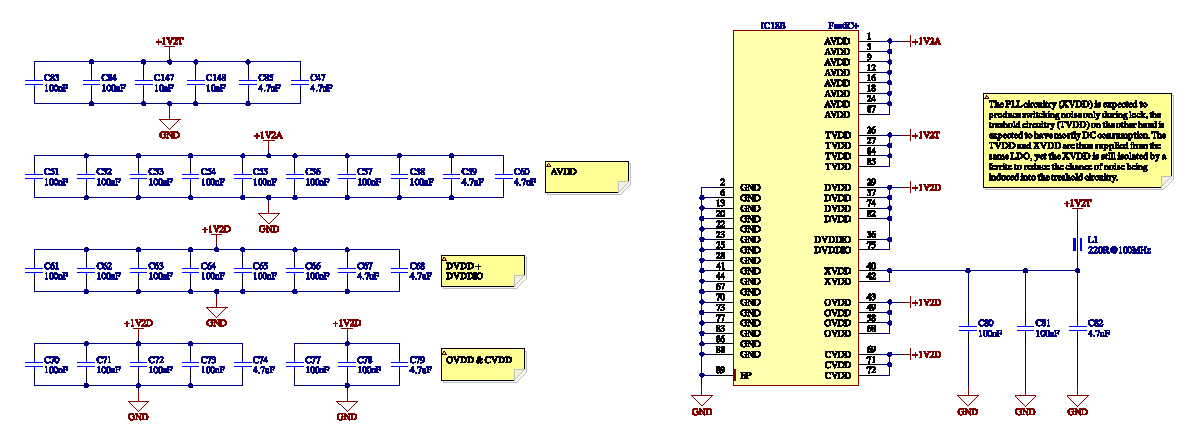
\includegraphics[scale=0.6]{schematic/fastic_power.eps}
    \caption{Schematic of the FastIC+ power}
    \label{fig:fastic_power}
\end{figure}
\FloatBarrier
%
To increase the stability of the internal band gap reference, a \SI{10}{\nano\farad} capacitor has been added to the \verb|VBG| pin.

Both \verb|nRST| (reset of the FastIC+) and \verb|SRST| (reset of the synchronous counter) have been pulled up to the digital supply so that the microcontroller pins in open drain mode can be used to control these pins without the need for voltage translation. 

\FloatBarrier
\begin{figure}[htp!]
    \centering
    \includegraphics[scale=0.6]{schematic/fastic.eps}
    \caption{Schematic of the FastIC+ logic}
    \label{fig:fastic}
\end{figure}
\FloatBarrier


%
\subsection{I2C communication}
As the FastIC+ voltage domains all run at \SI{1.2}{\volt}, a voltage shifter had to be implemented for communication with the microcontroller over I2C. For this, the PCA9306DQER has been chosen for its miniature X2SON package and sufficent \SI{400}{\kilo\hertz} speed. 
%
\subsection{Calibration pulse generator}
The FastIC+ features a \verb|CAL| input pin used for injecting a test pulse into any of the eight input channels. This pin converts the pulse to current with an internal \SI{70}{\ohm} resistor. The usual shape of such a pulse should resemble a real sensor output, thus a decaying exponential with an amplitude of a few milliamperes and length under a microsecond. To create this pulse, a high side switch has been implemented with series resistance to limit the current and parallel capacitance to recreate the decaying exponential. The transistor gate is driven by a quick digital pulse from the microcontroller, whos length can be adjusted to adjust the current pulse width and by some degree also the amplitude. 
%
\subsection{Voltage monitoring}
%
The \verb|VMON| pin on the ASIC serves for monitoring of the internal analog tresholds and DAC outputs. Since the microcontrollers internal voltage reference has been selected to run at \SI{1.8}{\volt}, a simple non inverting amplifier, with a voltage gain of
%
\begin{equation}
    A_V = \left( 1 + \frac{R41}{R44}\right) = \left( 1 + \frac{\SI{10}{\kilo\ohm}}{\SI{20}{\kilo\ohm}}\right) = 1.5
\end{equation}
%
has been implemented to amplify the \SI{1.2}{\volt} output to the microcontrollers full-scale range and improve the performance. Because the \verb|VMON| output is used only for treshold monitoring, thus only DC voltages, a slow RC filter has been used to reduce the noise coupled to the analog signal.
%
\FloatBarrier
\begin{figure}[htp!]
    \centering
    \includegraphics[scale=2]{schematic/fastic_vmon.eps}
    \caption{Schematic of the voltage monitoring amplifier}
    \label{fig:fastic_vmon}
\end{figure}
\FloatBarrier
%
\subsection{High speed outputs}
%
The FastIC+ outputs are realized using the Scalable Low Voltage Signaling standard. SLVS is a alternative to the LVDS, utilizing lower voltages. The transmitter common mode voltage $V_{CMTX}$ being \SI{0.6}{\volt} and the differential voltage $|V_{OD}|$ being \SI{0.2}{\volt} as seen in figure \ref{fig:slvs_voltages}.

\begin{figure}[ht]
	\begin{center}
		\includegraphics[scale=0.8]{06_SLVS_specs.pdf}
	\end{center}
	\vspace{-5mm}
	\caption{Voltage definition for SLVS transmitter.}
	\label{fig:slvs_voltages}
\end{figure}

A differential output capable of transmitting a pulse whos beginning timestamps the ToA of a photon and length resembles the ToT is present for each channel separately. However, as the readout uses the data digitalized by the internal TDC, these channels are left unconnected and disabled in the chip.

The \verb|TIME| output can either be used to generate a digital pulse whenever any input is received on any of the channels or can be internally connected to the trigger comparator and used for trigger calibration routine, the latter being used in this case. When the pin is not used for calibration, it is disabled to reduce any EMI generated by the fast edges. The \verb|TDCOUT| is the output of the Aurora stream from the transmitter.

Both of the above mentioned pins are connected to the DS90LVRA2 dual channel differential line receiver and terminated by a \SI{100}{\ohm} resistance. This receiver, used to convert the SLVS output to CMOS, has been chosen specifically for its small size, high enough speed but also for its typical propagation delay $t_{pd}$ = \SI{4.4}{\nano\second} to correctly align the data to the sampling clock. Even though it is made to convert LVDS signals, the treshold voltage levels work well with the SLVS standard mentioned above, thus no other special circuitry is needed. 

\subsection{Trigger input and output}
The trigger inputs (used for externally triggering the ASIC) and outputs (outputting the signal from the internal comparator) have been exposed to the user on two SMA connectors. Termination has been placed on these to mitigate any reflections and ESD protection diodes have been added to protect the chip from electrostatic discharge. It's important to note that the ESD diodes add capacitance to the trigger lines, thus degrading (slowing) the trigger edge and introducing a slight delay in the trigger. This either needs to be accounted for when using the readout or the diodes need to be left unassembled at the expense of worse ESD immunity. 
%
\FloatBarrier
\begin{figure}[htp!]
    \centering
    \includegraphics[scale=1.6]{schematic/fastic_top.eps}
    \caption{Schematic of the FastIC+ trigger circuitry}
    \label{fig:schem_fastic_triggers}
\end{figure}
\FloatBarrier

\section{USB}
To supply power to the device and handle communication with the host computer, a USB type C connector has been used.
\FloatBarrier
\begin{figure}[htp!]
    \centering
    \includegraphics[scale=.75]{schematic/usb_con.eps}
    \caption{Schematic of the USB connector with ESD protection}
    \label{fig:schem_usb_con}
\end{figure}
\FloatBarrier
\subsubsection{External PHY}
Because the combined data rate of the FastIC+ chips of \SI{160}{\mega\bit\per\second} exceeds the USB 1.1 specification, a USB 2.0 (High Speed) was implemented, supporting up to \SI{480}{\mega\bit\per\second} throughput. Unfortunately, the used microcontroller does not integrate the USB 2.0 PHY directly. Instead, it only integrates the necessary logic and interfaces with an external PHY via the ULPI interface. 


A USB3320 interface was chosen as it is well supported by the microcontroller and widely used in countless designs. A \SI{48}{\mega\hertz} crystal oscillator has been used as the external reference clock required for the device to operate. Different crystal frequency selection has been made possible with \SI{0}{\ohm} resistor jumpers. The ULPI connections have been series terminated, to better match the driver output impedance to the cotrolled impedance of the line. 
\FloatBarrier
\begin{figure}[htp!]
    \centering
    \includegraphics[scale=.68]{schematic/usb.eps}
    \caption{Schematic of the USB}
    \label{fig:schem_usb}
\end{figure}
\FloatBarrier
\subsubsection{Power Delivery}
A FUSB302 chip was added to allow for power limit negotiation with a UCPD capable power source. The chip handles all the necessary signaling and communicates with the MCU via a I2C interface. Optional \SI{5.1}{\kilo\ohm} resistors have been added to passively negotiate the highest power limit, if it would be decided to omit the power delivery functionality and not assemble the FUSB302.
\FloatBarrier
\begin{figure}[htp!]
    \centering
    \includegraphics[scale=.9]{schematic/ucpd.eps}
    \caption{Schematic of the USB}
    \label{fig:schem_ucpd}
\end{figure}
\FloatBarrier
\subsection{Clock generation}
For generating the \SI{40}{\mega\hertz} reference clock for both of the FastIC+ chips and the \SI{80}{\mega\hertz} sampling clock for the SPI peripherals, the SI5340 clock synthetizer has been used. It features four outputs with \SI{90}{\femto\second} RMS jitter, supporting both CMOS and differential output. Additionally, each output can be powered by an independent power supply allowing for mixing the \SI{3.3}{\volt} CMOS signals for the microcontroller and differential signals for the FastIC+. A precise \SI{48}{\mega\hertz} crystal oscillator has been used as the reference clock. The chip features both I2C and SPI interface for configuration. I2C was selected to be used in this design.

\FloatBarrier
\begin{figure}[htp!]
    \centering
    \includegraphics[scale=0.65]{schematic/clock.eps}
    \caption{Schematic of the clock generator}
    \label{fig:schem_clock}
\end{figure}
\FloatBarrier

Since the FastIC+ requiers an SLVS input, which is not supported by the generator a signal divider had to be implemented. This circuit, shown in figure \ref{fig:schem_slvs}, was provided in the datasheet as a good way to lower the voltage levels while keeping the impedance of the lines well matched. 
\FloatBarrier
\begin{figure}[htp!]
    \centering
    \includegraphics[scale=2]{schematic/slvs.eps}
    \caption{Divider for the LVDS to SLVS conversion}
    \label{fig:schem_slvs}
\end{figure}
\FloatBarrier

\subsection{High Voltage}
All the sensors, which the FastIC+ shall interface with, like SiPMs, PMTs or MCPs need high voltage biasing for their function. To eliminate the need for an external HV supply, an internal one has been implemented using the LT3571. This DC/DC converter, intended for biasing of avalanche photodiodes, is capable of generating up to \SI{75}{\volt} output from a low voltage input. It fully integrates the power switch and regulation along with soft-start and variable switching frequency. This has been set to approximately \SI{1}{\mega\hertz} via \verb|R61|. Higher switching frequency than allows for use of smaller inductance and thus keep the size of the device small. 

\FloatBarrier
\begin{figure}[htp!]
    \centering
    \includegraphics[scale=.65]{schematic/hv.eps}
    \caption{High voltage power supply schematic}
    \label{fig:schem_hv}
\end{figure}
\FloatBarrier

A \verb|CTRL| input is available for adjusting the output with a control voltage. This reference is generated by the MCU DAC and divided by a voltage divider to a suitable \SI{0}{V} -  \SI{1}{V} range. The feedback resistor divider was chosen such that the theoretical maximum output voltage with the \verb|CTRL| pin held at \SI{1}{\volt} is \SI{84.3}{\volt} according to equation \ref{eq:hv_voltage_fb}.

\begin{equation}
V_{MONIN} = (\frac{R57}{R62} + 1) \cdot V_{CTRL} = (\frac{\SI{1000}{\kilo\ohm}}{\SI{12}{\kilo\ohm}} + 1) \cdot \SI{1}{\volt} = \SI{84.3}{\volt}
\label{eq:hv_voltage_fb}
\end{equation}


The current limit resistor has been chosen to limit the APD current to approximately \SI{8}{\milli\ampere} based on the equation \ref{eq:hv_current_limit} mentioned in the datasheet.

\begin{equation}
R_{SENSE} = \frac{\SI{200}{\milli\volt}}{1.2 \cdot I_{APD} + \SI{0.3}{\milli\ampere}} \approx \SI{20}{\ohm}
\label{eq:hv_current_limit}
\end{equation}
%
where $I_{APD}$ is the APD current limit in milliamperes.

To allow for closed loop control with the microcontroller, the output voltage on the APD pin is monitored via a suitable voltage divider with an operational amplifier buffer. For current monitoring, the LT3571 offers the \verb|IMON| pin which sources a current $I_{IMON} = 0.2 \cdot I_{APD}$. This current is than converted to voltage with a \SI{1}{\kilo\ohm} shunt resistor and buffered with an operational amplifier.

\FloatBarrier
\begin{figure}[htp!]
    \centering
    \includegraphics[scale=.8]{schematic/hv_isense.eps}
    \includegraphics[scale=.8]{schematic/hv_usense.eps}
    \caption{Sensing of the high voltage and current}
    \label{fig:schem_hvsense}
\end{figure}
\FloatBarrier

\subsection{Power}
A DC/DC converter has been implemented to efficiently lower the \SI{5}{\volt} input voltage to the \SI{3.3}{\volt} used by the microcontroller. The \SI{3.3}{\volt} for the analog domain has been generated with a low ripple LDO. The \SI{1.8}{\volt} domain for the USB interface has been derived from the \SI{3.3}{\volt} using an LDO aswell, as efficiency is not required with the low power consumption of \SI{29.4}{\milli\ampere} of the \SI{1.8}{\volt} domain.
\FloatBarrier
\begin{figure}[htp!]
    \centering
    \includegraphics[scale=1]{schematic/power_dcdc.eps}
    \caption{Step down regulator schematic}
    \label{fig:schem_dcdc}
\end{figure}
\FloatBarrier

Power sequencing has been implemented for all the three FastIC+ voltage domains. First, the digital domain supply is activated, followed by the supply for the treshold circuitry and PLL and lastly, the analog domain is supplied. All of these domains are derived from the \SI{3.3}{\volt} using a \SI{1.2}{\volt} LDOs which are sufficient for the low power consumption (\SI{113}{\milli\ampere} per chip) and provide a ripple-free supply for the sensitive treshold circuitry.

\FloatBarrier
\begin{figure}[htp!]
    \centering
    \includegraphics[scale=.55]{schematic/power_fastic.eps}
    \caption{FastIC+ power domain sequencing}
    \label{fig:schem_fastic_power}
\end{figure}
\FloatBarrier

\section{Connector}
For interfacing with the user board, the \SI{9}{\milli\meter} high version of ERM8-020 has been used for its durability, up to 1000 connection cycles, good high speed performance and suitable pin count. This connector carries all the sixteen input channels alongside the high voltage biasing supply. The \SI{3.3}{\volt} supply is also exposed and four pins are dedicated to the user board identification.
%
\subsubsection{Identification pins}
The identification pins serve as an easy way to assign a four bit short ID to a specific user board. This ID can than be used by the software to load a configuration preset defined for the user board. If the userboard designer decides to, the pins ID0 and ID1 can be used as I2C communication lines. A compatible EEPROM can than be assembled on the user board, making it possible to save the full configuration on the user board itself, as well as additional data such as name or a unique ID. If the I2C interface is to be used, all of the ID pins need to be pulled up high by a suitable resistor. At least one of the ID pins has to be high at all times, this means that an ID of \verb|0b0000| is not allowed and in this case, the readout will not recognize a valid user board. 
%
\chapter{Userboard}
The userboard has been developed as a template for the users to get easily started with the readout system. It contains a matrix of 4 $\times$ 4 SiPM sensors as well as an EEPROM for storing the board configuration. The \SI{9}{\milli\meter} high ERF8-020 connector has been chosen for the user board to match the counterpart present on the readout and allow enough clearance between the assembled readout board and user board.

\section{Sensors}
The footprint for a generic THT SiMPs has been implemented on the board. Each SiPM is powered from the HV plane and the input is filtered with a dual RC low pass to eliminate a possibility of cross triggering of the sensors. 

\FloatBarrier
\begin{figure}[htp!]
    \centering
    \includegraphics[scale=1.2]{schematic/sipm.eps}
    \label{fig:sipm}
\end{figure}
\FloatBarrier

\section{EEPROM}
The 24AA04T-I/OT \SI{4}{\kilo\bit} EEPROM has been used on the user board for the configuration storage. It has been selected for the low price and sufficient capacity. 



\newpage
\chapter{PCB design}
Special care had to be taken when designing the PCB to keep in mind the correct design practices for propper power integrity, signal integrity and high speed design.

First a suitable stackup was chosen. In this case, it was decided to proceed with an eight layer stackup as shown in table \ref{tab:stackup}. 
\FloatBarrier
\begin{table}[]
    \caption{PCB stackup}
    \begin{tabular}{|l|l|l|}
    \hline
    \multicolumn{1}{|c|}{\textbf{Layer}} & \multicolumn{1}{c|}{\textbf{Name}} & \multicolumn{1}{c|}{\textbf{Thickness}} \\ \hline
    1                                    & L1 - Top copper                    & \SI{0.018}{\milli\meter}                                   \\ \hline
                                         & Dielectric - PR2116                & \SI{0.120}{\milli\meter}                                   \\ \hline
    2                                    & L2 - Ground plane                  & \SI{0.035}{\milli\meter}                                   \\ \hline
                                         & Dielectric - FR4 core              & \SI{0.200}{\milli\meter}                                   \\ \hline
    3                                    & L3 - Power plane                   & \SI{0.035}{\milli\meter}                                   \\ \hline
                                         & Dielectric - PR2116                & \SI{0.120}{\milli\meter}                                   \\ \hline
                                         & Dielectric - PR2116                & \SI{0.120}{\milli\meter}                                   \\ \hline
    4                                    & L4 - Signal layer                  & \SI{0.035}{\milli\meter}                                   \\ \hline
                                         & Dielectric - FR4 core              & \SI{0.200}{\milli\meter}                                   \\ \hline
    5                                    & L5 - Signal layer                  & \SI{0.035}{\milli\meter}                                   \\ \hline
                                         & Dielectric - PR2116                & \SI{0.120}{\milli\meter}                                   \\ \hline
                                         & Dielectric - PR2116                & \SI{0.120}{\milli\meter}                                   \\ \hline
    6                                    & L6 - Power plane                   & \SI{0.035}{\milli\meter}                                   \\ \hline
                                         & Dielectric - FR4 core              & \SI{0.200}{\milli\meter}                                   \\ \hline
    7                                    & L7 - Ground plane                  & \SI{0.035}{\milli\meter}                                   \\ \hline
                                         & Dielectric - PR2116                & \SI{0.120}{\milli\meter}                                   \\ \hline
    8                                    & L8 - Bottom copper                 & \SI{0.018}{\milli\meter}                                   \\ \hline
    \end{tabular}
    \label{tab:stackup}
\end{table}
\FloatBarrier
The layers 2 and 3 and layers 6 and 7 were completly dedicated as ground and power planes. This, in combination with relatively thin dielectric in between, creates an inherent capacitive coupling between the planes proportional to the plane area and spacing which helps the power integrity of the device. For a board of size $\SI{50}{\milli\meter} \times \SI{50}{\milli\meter}$, which is the case for the readout, and the stackup mentioned, this capacitance can be estimated with an equation for a parallel plate capacitor to be
%
\begin{equation}
C = \varepsilon_0 \cdot \varepsilon_r \cdot \frac{S}{d} = \SI{8.85e-12}{\farad\per\meter} \cdot 4.2 \cdot \frac{\SI{2500}{\milli\meter\squared}}{\SI{0.2}{\milli\meter}} = \SI{46.5}{\pico\farad}
\end{equation}
%
Leaving the planes for solid planes only also keeps the impedance of the planes minimal which reduces the voltage drops in the planes. The layers 4 and 5 were also mostly kept as planes, although some connections needed to be routed through these because of the very high board density. While routing in these layers, care was taken not to cross possible return current paths of the planes with another trace, which could result in a much bigger current loop and an increase in EMI. Layers 1 and 8, the top and bottom copper, were used mainly for routing of all the signals. Since both of the layers have a ground reference underneath, both of them can and were used for routing of the high speed lines with defined impedance. 
%
\section{High speed signals}
To mitigate any possible reflections on the high speed lines which carry high frequency signals, the charasteristic impedance of all of these was calculated to match the driver impedance. In case of the differential signals, the differential impedance of the lines was optimized to be \SI{100}{\ohm}, aside from the USB which requires a \SI{90}{\ohm} differential impedance. For the single ended lines, the target impedance was \SI{50}{\ohm}. The widths of the lines along with the spacing for the differential lines were calculated using the Altium Designer impedance calculation tool and double checked using the manufacturers impedance calculation tool. These calculations yilded the width $W_{USB} = \SI{11111}{\milli\meter}$ and spacing $S_{USB} = \SI{11111}{\milli\meter}$ for the USB differential pair, the width $W_{DIFF} = \SI{0.15}{\milli\meter}$ and spacing $S_{DIFF} = \SI{0.2}{\milli\meter}$ for the rest of the differential pairs and the width $W_{SE} = \SI{0.182}{\milli\meter}$ for all of the single-ended high speed lines. The widths and spacings were obeyed during the routing to keep the tracks impedance as close to the target impedance as possible.

\section{BGA fanout}


\section{Power integrity}

The two concepts described above were designed and manufactured keeping in mind the required performance. The final PCBs can be seen on the images bellow. 
\newpage
\FloatBarrier
\begin{figure}[htp!]
    \centering
    \includegraphics[height=5.2cm]{readout_3d-top.png}
    \includegraphics[height=5.2cm]{readout_3d-bottom.png}
    \caption{Readout PCB}
    \label{fig:readout_3d}
\end{figure}
\FloatBarrier

\FloatBarrier
\begin{figure}[htp!]
    \centering
    \includegraphics[height=5.2cm]{userboard_3d-top.png}
    \hspace{1.8cm}
    \includegraphics[height=5.2cm]{userboard_3d-bottom.png}
    \caption{Userboard PCB}
    \label{fig:userboard_3d}
\end{figure}
\FloatBarrier

\chapter{Enclosure Design}
To complete the device design, a custom enclosure was created to house both the readout PCB and the user board. The enclosure is designed to protect the sensitive electronics while ensuring adequate airflow for thermal management. It consists of three main components: 

\begin{itemize}
    \item \textbf{Bottom Shell}: This part includes holes for the reset button, boot button, and LED indicator.
    \item \textbf{Sleeve}: This section features cutouts for all the SMA connectors and the USB port.
    \item \textbf{Top Shell}: This piece fully encloses the readout PCB.
\end{itemize}

Holes for metal heat inserts are located in the corners. Once the inserts are in place, the three parts are secured together using four M2 screws. The user board can be easily disconnected from the readout PCB. If needed, it can also be fixed in place using M2 screws. The placement of the inserts and screws is depicted in Figure \ref{fig:readout_inserts}.

\FloatBarrier
\begin{figure}[htp!]
    \centering
    \includegraphics[height=4cm]{insert.png}
    \caption{Metal insert placement}
    \label{fig:readout_inserts}
\end{figure}
\FloatBarrier

The enclosure was designed to be 3D printed using a standard \emph{FDM} printer. The top shell and sleeve can either be printed separately and glued together, or they can be printed as a one piece on multi material printer. The design process was carried out in Fusion 360. Renders of the enclosure are shown below.

\FloatBarrier
\begin{figure}[htp!]
    \centering
    \includegraphics[height=8cm,trim={11cm 0 11cm 0},clip]{mech_preview.png}
    \caption{3D Preview of the Readout PCB Enclosure}
    \label{fig:readout_3d_preview}
\end{figure}
\FloatBarrier

\FloatBarrier
\begin{figure}[htp!]
    \centering
    \includegraphics[height=6cm]{mech_top.png}
    \includegraphics[height=6cm]{mech_bottom.png}
    \includegraphics[height=6cm]{mech_front.png}
    \includegraphics[height=6cm]{mech_rear.png}
    \caption{Top, Bottom, Front, and Rear Views of the Enclosure}
    \label{fig:readout_3d_views}
\end{figure}
\FloatBarrier

\chapter{Firmware}
A firware in the C++ programming language has been developped for the readout aiming for best performance and reliable functionality. 
\section{USB}
The TinyUSB library has been used for implementing the USB stack on the device. It is an open-source cross-platform USB stack for embedded systems, designed to be memory-safe with no dynamic allocation and thread-safe. It provides support for both Host and Device roles and implements all the common usb classes such as CDC, HID, DFU, Vendor specific and others. On the STM32H7 series specifically, it is capable of working with the ULPI PHY in HS mode and make use of the internal DMA to allow for very high throughput and good latency. All of these specification make it ideal for this application.

Three interfaces have been implemented in order to allow for configuration of the device via human readable protocol, binary protocol and readout of the two data streams.
\subsection{CDC interface}
A Communication Device Class has been implemented on the first interface (endpoints 0x81, 0x82 ans 0x02). This interface emulates a COM port over USB and allows for easy, human-readable interaction with the device. A simple text protocol has been impemented to serve all the required functions of the device. 
\newpage
The following commands have been implemented, where square brackets indicate a choice between the options separated by slash and curly braces indicate value in the specified format:
%
\begin{itemize}
    \item \verb|get readout status| - returns the status of the readout
    \item \verb|get readout uid| - returns a UID of the readout
    \item \verb|get hv enable| - returns the state of the HV supply
\end{itemize}
\begin{verbatim}
set hv enable [true/false]
get hv current
get hv voltage
set hv voltage {float: voltage}
get fastic register [1/2] {hex byte: address}
set fastic register [1/2] {hex byte: address} {hex byte: value}
get fastic voltage [1/2]
get fastic syncreset [1/2]
set fastic syncreset [1/2] [high/low]
set fastic calpulse [1/2] [enable/disable]
get fastic time [1/2]
get fastic aurora [1/2]
set fastic aurora [1/2] [enable/disable]
get userboard status
get userboard uid
get userboard name
set userboard name {string: name}
get userboard writeprotect
set userboard writeprotect [true/false]
get userboard init
set userboard init 
get userboard voltage 
set userboard voltage {float: voltage}
get userboard register [1/2] {hex byte: address}
set userboard register [1/2] {hex byte: address} {hex byte: value}
set userboard tomemory
set userboard frommemory
\end{verbatim}

A detailed description of the commands and their usage is provided in the device user manual.

\subsection{Vendor control}
The USB specification describes a way to communicate with a USB device in a bursty matter by Control Transfers. A control transfer is typically a short random packet, containing up to \SI{64}{\byte} of data, which is delivered to the default endpoint with the best effort delievery (no retransmissions). These packets are, for example, used to control the flow of the CDC interface but can be very easilly adopted to transfer auxilary vendor data and thus allow for binary communication with the device. 

The same commands as in the CDC interface have been implemented using control transfers to allow for easier interactions with the device via software on the PC as the text communication adds unneccessary overhead in thios regard.

A control transfer is started by an eight byte long Setup Packet, which contains the following fields:

\FloatBarrier
\begin{figure}[htpb]
    \begin{center}
        \begin{bytefield}[endianness=little,bitwidth=1em]{32}
            \bitheader{0,7,8,15,16,31} \\
            \bitbox{8}{\texttt{\footnotesize bmType}} & 
            \bitbox{8}{\texttt{\footnotesize bRequest}} & 
            \bitbox{16}{\texttt{\footnotesize wValue}} \\[3ex]
            \hfill
            \bitheader[lsb=32]{32,47,48,63} \\
            \bitbox{16}{\texttt{\footnotesize wIndex}} & 
            \bitbox{16}{\texttt{\footnotesize wLength}} 
        \end{bytefield}
        \caption{Setup packet structure}
        \label{fig:usb_control_transfer}
    \end{center}
\end{figure}


\verb|bmType| indicates the direction of the communication, the type, in this case a Vendor transfer, and the recipient, in this case a Device. \verb|bRequest| field indicates the request number. The readout text commands have been each mapped to a unique number which is used in this field in the binary communication. \verb|wValue| and \verb|wIndex| allow for other parameters to be passed with the request, in this case parameters such as the index of the FastIC+ chip to work with. If there is more data to be transfered, the \verb|wLength| field is used to specify the length of an additional data packet sent after the Setup Packet.

\subsection{Vendor interfaces}
For transfering the Aurora data stream from the FastIC+ chips to the computer, two vendor interfaces have been implemented, one for each FastIC+ chip. The sampled bitstream is transfered using Bulk Transfers over these two interfaces. 

\section{Clock generation}
The configuration for the Si5340 clock synthetizer was generated using the Clock Builder application provided by Skyworks. This software generates a register map as a C/C++ array that is later parsed by the software and the configuration is applied to the synthetizer over I2C.

\section{HV power supply}
For controlling the HV power supply, a DAC peripheral has been used to provide the control voltage. Two channels of an ADC peripheral with 256 times oversampling, resulting in a \SI{1000}{\sample\per\second} sample rate were used. 
\subsection{PID tuning}

\section{FastIC+}
\subsection{I2C Communication}
\subsection{Aurora stream}
\subsection{Pulse injection}

\section{Userboard}

\chapter{Software}
A simple Python-based software application was developed to handle basic user tasks. Python was chosen for its simplicity, ease of use, and widespread adoption within the scientific community. However, this choice comes with certain drawbacks, such as reduced performance, which becomes noticeable when processing large amounts of data, such as binary streams from the FastIC+. To address this, efforts were made to optimize the code for speed wherever possible.
\section{Device communication}
The first component of the software is a library of functions for communicating with the device via vendor control transfers and for reading FastIC+ data streams into binary files. The `pyusb` library was utilized for both vendor control transfers and bulk data transfers.

\section{Stream processing}
The second component is a library designed to process the captured data. This library handles synchronization, decoding, and parsing of the data, ultimately outputting FastIC+ packets as objects. It aligns the bitstream using detected Aurora synchronization preambles, reads the block data, descrambles it, and assembles it into packets.

\section{Example scripts}
Finally, these two components were integrated into a simple example script. This script configures the FastIC+ parameters, sets up the HV bias, captures a sample data stream, and decodes it and exports the decoded packets to the user. Additional functionality, such as the comparator calibration procedure, remains to be implemented. These tasks are left either to the users or to the FastIC+ researchers, who, with their in-depth knowledge of the chip, can provide the most efficient implementations.

\chapter{Function verification}
To verify the functionality of the device, a serie of basic measurements was performed. Later on a more complex test - injecting synthetised pulses to the fastic - was performed and the functionality of the whole device was thus verified.
\section{Measurements}
Multiple measurements were done to verify the basic functionality of the device. A \SI{200}{\mega\hertz} DSO-X 2024A oscilloscobe with a \SI{350}{\mega\hertz} probe has been used to carry out the measurements. Measurements on the power supplies were done as close to the supply output as possible. A spring contact was used to contact the ground of the probe to minimize the loop inductance of the probe.
\subsection{Power supplies}
The output ripple of the step down DC/DC converter was measured to be \SI{26}{\milli\volt} peak-to-peak. The frequency of the ripple measured coresponds well to the switching frequency of the converter (\SI{750}{\kilo\hertz}) \cite{diodes_ap62201} which can be seen in Figure \ref{fig:dcdc_ripple}. Note that the cursor frequency is measured over the span of 5 periods to get better accuracy, thus the measured value has to be multiplied by 5. For the LDOs, there was no observable ripple on the output. Both of these confirm that the power network integrity of the device is very good.

\FloatBarrier
\begin{figure}[!htpb]
    \begin{center}
        \includegraphics[height=6cm]{measurements/dcdc_ripple.png}
        \caption{Output ripple of the DC/DC converter}
        \label{fig:dcdc_ripple}
    \end{center}
\end{figure}
\FloatBarrier

\subsection{High Voltage power supply}
Next, the output voltage ripple of the high voltage power supply was measured at \SI{20}{\volt} with a \SI{100}{\kilo\ohm} load connected. The transient response to this load was also measured. 
\FloatBarrier
\begin{figure}[!htpb]
    \begin{center}
        \includegraphics[height=6cm]{measurements/ripple.png}
        \caption{Output ripple of the high-voltage power supply}
        \label{fig:hv_ripple}
    \end{center}
\end{figure}
\FloatBarrier

\FloatBarrier
\begin{figure}[!htpb]
    \begin{center}
        \includegraphics[height=6cm]{measurements/hv_transient.png}
        \caption{Trensient response of the high-voltage power supply}
        \label{fig:hv_transient}
    \end{center}
\end{figure}
\FloatBarrier

From Figure \ref{fig:hv_ripple}, it can be seen that a ripple of \SI{45}{\milli\volt} peak-to-peak was observed, which is low enough to avoid causing any issues with the biased sensors. These sensors will experience an even cleaner supply voltage due to the low-pass filtering. Figure \ref{fig:hv_transient} shows the transient response of the power supply. When the load is connected, the output voltage drops by \SI{100}{\milli\volt} and takes \SI{150}{\micro\second} to stabilize back to the setpoint. This will not cause any problems, as this voltage drop is small enough to avoid triggering any other sensors. The typical pulse from the connected sensor will also be much shorter, on the order of a few hundred nanoseconds, causing a much smaller voltage drop. Thus, the evaluated case represents a worst-case scenario.

\subsection{Pulse injection}
The function of the pulse injection circuitry was also verified by measurement, which can be seen in Figure \ref{fig:injection_meas}. The peak voltage of \SI{3.16}{\volt} corresponds to a current of approximately \SI{10}{\milli\ampere} through the front end. The width of the pulse was set to \SI{200}{\nano\second}.

\FloatBarrier
\begin{figure}[!htpb]
    \begin{center}
        \includegraphics[height=6cm]{measurements/injection.png}
        \caption{Injected pulse}
        \label{fig:injection_meas}
    \end{center}
\end{figure}
\FloatBarrier

\section{Injection pulse test}
For the injection pulse test, the FastIC+ 1 was configured to enable the injection signal routing into channel 0. The injection pulse generator was than enabled to generate the injection signal (\SI{100}{\nano\second} pulses with \SI{100}{\micro\second} period). Streaming of the aurora data to the USB was than started and \SI{100}{\milli\second} capture of the bitsream was created. The python library was than used to parse the raw data into packets. The packets for a first packet detection is presented bellow.
\begin{small}
\begin{verbatim}
    --- Packet 1 ---
    Channel: 0
    Packet Type: PKT_TOTLN
    Timestamp absolute: 107474.438 us
    Pulse Width: 106.249 ns
  
    --- Packet 2 ---
    Channel: 8
    Packet Type: PKT_TOA_TOTNL
    Timestamp absolute: 107474.251 us
    Pulse Width: 1032.812 ns
  
    --- Packet 3 ---
    Channel: 0
    Packet Type: PKT_TOA
    Timestamp absolute: 107474.247 us
    Pulse Width: 124.218 ns

\end{verbatim}
\end{small}
\newpage
Along with a second detection that is subsequent to the fist one.
\begin{small}
\begin{verbatim}
    --- Packet 1 ---
    Channel: 0
    Packet Type: PKT_TOTLN
    Timestamp absolute: 107572.038 us
    Pulse Width: 107.031 ns
  
    --- Packet 2 ---
    Channel: 8
    Packet Type: PKT_TOA_TOTNL
    Timestamp absolute: 107571.850 us
    Pulse Width: 1035.546 ns
  
    --- Packet 3 ---
    Channel: 0
    Packet Type: PKT_TOA
    Timestamp absolute: 107571.846 us
    Pulse Width: 125.000 ns
  
\end{verbatim}
\end{small}

The two packets received on channel 0 correspond to the \emph{ToA} of the pulse, transferred in the \verb|PKT_TOA| packet, and the \emph{ToT} transferred in the \verb|PKT_TOTLN|. The third packet on channel 8 is the \emph{ToA} of the trigger pulse generated to start the FSM. These differ due to different thresholds and processing on the separate paths. Taking the relevant information from the first set, it can be seen that a packet with a \emph{ToT} of \SI{106.249}{\nano\second} was detected at time \SI{107474.247}{\micro\second}. The \emph{ToT} corresponds nicely to the generator pulse width. Taking the difference between the \emph{ToA} timestamps of the subsequent detections, the period of the pulses can be calculated as $T = \SI{107571.846}{\micro\second} - \SI{107474.247}{\micro\second} = \SI{97.599}{\micro\second}$, which corresponds to the set period of \SI{100}{\micro\second} of the injection generator. The inaccuracy of both the \emph{ToA} and \emph{ToT} originates from the injection generator rather than the FastIC+, which is very precise. The purpose of the injection is to easily check that the FastIC+ can receive pulses and process them correctly, rather than verifying the FastIC+'s accuracy. 


\section{SiPM SPTR measurement}
To verify the device's functionality in a real-world application and stress test the FastIC+ accuracy, a Single Photon Time Resolution (SPTR) measurement with a real SiPM was performed at CERN. In this test, a laser source sends short pulses of light to a \emph{SiPM} sensor connected to the readout. A trigger signal output from the laser is fed into the readout trigger input. On every laser shot, the readout is triggered by the laser and thus generates a \emph{ToA} packet on channel 8. After the beam of light travels to the \emph{SiPM}, it is converted into an electrical pulse and sensed by the FastIC+, which generates the \emph{ToA} and \emph{ToT} packets for the detection. The delay between the trigger \emph{ToA} and the detection \emph{ToA} corresponds to the time the \emph{SiPM} needs to detect the photon and generate the electrical pulse, thus the \emph{SPTR} of the \emph{SiPM}. The \emph{ToT} is used to detect only single-photon events. 
\\
\\
\large \textbf{TADY BUDE DALSI KOMENTAR K TOMU EXPERIMENTU AZ HO CERN UDELA :D}



\clearpage
\FloatBarrier
\printbibliography

\chapter*{List of abbreviations}
\noindent
\begin{tabularx}{\linewidth}
{ l >{\raggedright\arraybackslash}X }
\bfseries Abbreviation & \bfseries Explanation\\\Midrule
CERN & Conseil Européen pour la Recherche Nucléaire \\
ASIC & Application Specific Integrated Circuit \\
PET & Positron Emission Tomography\\
TDC & Time-to-Digital Converter\\
SiPM & Silicon Photo Multiplier\\
PMT & Photo Multiplier Tube\\
MCP & Micro Channel Plate\\
ToA & Time of Arrival\\
ToT & Time over Threshold\\
ToF PET & Time of Flight Positron Emission Tomography\\
LIDAR & Light Detection and Ranging\\
I2C & Inter-Integrated Circuit\\
FSM & Finite State Machine\\
FERO & Front-End Readout\\
BERO & Back-End Readout\\
FIFO & First In First Out\\
MUX & Multiplexer\\
SLVS & Scalable Low Voltage Signaling\\
MSB & Most Significant Bit\\
LSB & Least Significant Bit\\
BTF & Block Type Field\\
USB & Universal Serial Bus\\
FPGA & Field Programmable Gate Array\\
HDL & Hardware Description Language\\
IP cores & Intellectual Property Cores\\
ADC & Analog to Digital Converter\\
DAC & Digital to Analog Converter\\
SPI & Serial Peripheral Interface\\
DMA & Direct Memory Access\\
TFBGA & Thin Fine Ball Grid Array\\
MCU & Microcontroller Unit\\
PLL & Phase Locked Loop\\
LVDS & Low Voltage Differential Signaling\\
CMOS & Complementary Metal-Oxide-Semiconductor\\
EMI & Electromagnetic Interference\\
SMA & SubMiniature version A\\
ESD & Electrostatic Discharge\\
PHY & Physical Layer\\
ULPI & UTMI+ Low Pin Interface\\
UTMI & USB Transceiver Macrocell Interface\\
UCPD & USB Type-C Power Delivery\\
RMS & Root Mean Square\\
LDO & Low Dropout Regulator\\
EEPROM & Electrically Erasable Programmable Read-Only Memory\\
THT & Through-Hole Technology\\
PCB & Printed Circuit Board\\
\end{tabularx}

\end{document}